\documentclass[12pt]{article}

\usepackage[utf8]{inputenc}
\usepackage{latexsym,amsfonts,amssymb,amsthm,amsmath}
\usepackage{tikz}
\usepackage{stanli}
\usetikzlibrary{shapes,calc,through,3d,patterns}
\usetikzlibrary{arrows.meta,decorations.pathreplacing,angles,quotes}
\usepackage{multicol}
\usepackage{geometry}
\usepackage{mathtools}
\usepackage{siunitx}
\usepackage{booktabs}

\setlength{\parindent}{0in}
\setlength{\oddsidemargin}{-0.25in}
\setlength{\textwidth}{7in}
\setlength{\textheight}{9.3in}
\setlength{\topmargin}{-1in}
\setlength{\headheight}{18pt}

\newcommand\blfootnote[1]{%
    \begingroup
    \renewcommand\thefootnote{}\footnote{#1}%
    \addtocounter{footnote}{-1}%
    \endgroup
}

\definecolor{darkred}{rgb}{0.6,0,0}

\newcommand{\bolddelta}{\boldsymbol\delta}
\newcommand{\boldxi}{\boldsymbol\xi}

\begin{document}

\noindent ME473 - Dynamic finite element analysis of structures\hfill EPFL\\
Stefano Burzio \hfill 2025\\
\vspace{0.3cm}

\hspace*{\fill}\textbf{\Large Problem set 3}\hspace*{\fill}

\hrulefill


\subsection*{Problem 1}
Consider the longitudinal vibrations of a bar of length \( \ell \), with a constant cross-sectional area \( A \), constant Young's modulus \( E \), and constant material density \( \rho \). The bar is fixed at the left end and free at the right end, as shown in the figure below.
\begin{center}
    \begin{tikzpicture}[scale=1]
        \point{a}{0}{0};
        \support {3}{a}[270];
        % Draw the rectangle
        \filldraw[fill=gray!40, draw=black,thick] (0,-0.5) -- (10,-0.5) -- (10,0.5) -- (0,0.5) -- cycle;
        %axis
        \draw[-latex, ultra thin] (0,0) -- (11.7,0) node[below] {\(x\)};
        \draw[ ultra thin] (0,-1.3) -- (0,1.3);
        % length
        \draw[ultra thin] (10,0) -- (10, 1.3) ;
        \draw[latex-latex, ultra thin]  (0,1)  to node[sloped,midway,above] {$\ell$}(10,1) ;
        \draw[ultra thin]  (7,-0.3) -- (8,-1) node[right]{$E,A,\rho$};
        \draw[ultra thick] (0,0) --(10,0);
        % Mark points
        \fill (0,0) circle (3pt) node[below right] {$x_1$};
        \fill (10,0) circle (3pt) node[below right] {$x_3$};
        \draw[fill=white, draw=black] (5,0) circle (3pt) node[below right] {$x_2$};
    \end{tikzpicture}
\end{center}
The longitudinal vibrations of the bar are governed by the following weak form: find the longitudinal displacement $u_1(\cdot,t) \in \mathcal U$, such that the following equation is satisfied for every $\delta u_1 \in \mathcal V$
\begin{equation*}
    \label{wf}
    \int_0^{\ell} E A\left(\frac{\partial u_1}{\partial x}\right)\left(\frac{\partial \delta u_1}{\partial x}\right)\, dx+
    \int_0^{\ell} \rho A \ddot{u}_1 \delta u_1\, dx=0
\end{equation*}
coupled with the initial conditions expressed in weak or integral form. Moreover, the functional spaces are defined as
\begin{align*}
    \mathcal U & =\big\{u_{1}(\cdot,t)\in H^1(]0,\ell[)\ |\  u_1(0,t)=0\ \forall t\in]0,T[\big\}, \\
    \mathcal V & =\big\{\delta u_{1}\in H^1(]0,\ell[)\ |\ \delta u_{1}(0)=0\big\}.
\end{align*}
Approximate the first and second natural frequencies using one quadratic finite element and compare the relative error with those obtained by exact analytical solution:
\begin{equation*}
    \omega_1^{\text{exact}} = \frac{\pi}{2} \sqrt{\frac{E}{\rho \ell^2}}\qquad\text{and}\qquad \omega_2^{\text{exact}} =\frac{3\pi}{2} \sqrt{\frac{E}{\rho \ell^2}}.
\end{equation*}
\textsc{Hint}: you can use \texttt{MATLAB} to calculate the coefficients of the stiffness and mass matrices.

\subsection*{Problem 2}
Consider a square rubber membrane, initially at rest at $t=0$, stretched between fixed supports, and subjected to a distributed transversal load $p$ while experiencing a uniform tension $S$. The weak formulation governing the transverse vibrations of the membrane is: find the transverse displacement  $u_3\left(x, y, t\right) \in\mathcal U$ such that the equation
\[
    -\int_{\Omega} S (\nabla \delta u_3)^{T}\nabla u_3 \, d\Omega + \int_{\Omega} p \delta u_3 \, d\Omega = \int_{\Omega} \rho \ddot{u}_3 \delta u_3 \, d\Omega,
\]
is satisfied for every virtual displacement $\delta u_3 \in\mathcal V$. The  initial conditions are given by
\[
    u_3(x, y, 0) = \dot{u}_3(x, y, 0) = 0.
\]
Notice that the initial displacement and initial velocity of the membrane are both set to zero. Here $\rho$ represents the density, $\Omega = ]0, \ell[ \times ]0, \ell[$ is the domain (rectangle of sides $a_1$ and $a_2$), and the nabla operator is defined as
\[
    \nabla= \begin{bmatrix}
        \partial / \partial x \\
        \partial / \partial y
    \end{bmatrix}.
\]
The functional spaces are defined as
$$\begin{aligned}
         & \mathcal U=\left\{ u_3(\cdot,t) \in H^1(\Omega) ; u_3(\cdot, t)=0 \text{ on } \Gamma\right\}, \\
         & \mathcal V=\left\{\delta u_3 \in H^1(\Omega) ; \delta u_3=0 \text{ on } \Gamma\right\},
    \end{aligned}$$
where $\Gamma$ is the boundary of the membrane.

\begin{center}
    \begin{minipage}[b]{.45\textwidth}
        \begin{tikzpicture}
            % Draw the rectangle (domain)
            \filldraw[fill=gray!40, draw=black,thick]  (0,0) -- (5,0) -- (7,2) -- (2,2) -- cycle;
            % Labels for dimensions
            \draw[ultra thin] (0,0) -- (-0.5,-0.5);
            \draw[ultra thin] (2,2) -- (1.3,2);
            \draw[ultra thin] (5,0) -- (4.5,-0.5);
            \draw[ultra thin,latex-latex] (-0.3,-0.3) -- (4.7,-0.3) node[midway, below] {$\ell$};
            \draw[ultra thin,latex-latex] (-0.5,0) -- (1.5,2) node[midway, left] {$\ell$};
            % Axes
            \draw[ultra thin,-latex] (-0.7,0) -- (6,0) node[right] {$x$};
            \draw[ultra thin,-latex] (-.5,-0.5) -- (2.7,2.7) node[above] {$y$};
            % Arrows representing force p
            \foreach \x in {1.5, 2.5, 3.5, 4.5}
                {
                    \draw[thick,latex-] (\x,.3) -- (\x,.8);
                    \draw[thick,latex-] (\x+.5,1.3) -- (\x+.5,1.8);
                }
            \node at (3,1) {$p$};

            % Labels
            \draw[ultra thin] (5.2,1) -- (7,3) node[right]{$\Omega, S, \rho$};
            \draw[ultra thin] (6,1) -- (7,1.5) node[right]{$\Gamma$};

        \end{tikzpicture}
    \end{minipage}
    \begin{minipage}[b]{0.45\textwidth}
        \begin{tikzpicture}
            % Draw the rectangle (domain)
            \filldraw[fill=gray!40, draw=black,thick]  (0,0) -- (5,0) -- (7,2) -- (2,2) -- cycle;
            %elements
            \draw[thick] (2.5,0) -- (4.5,2);
            \draw[thick] (1,1) -- (6,1);
            \draw[ultra thin] (1.5,0.5) -- (-.5,1)node[left]{${}^1\Omega$};
            \draw[ultra thin] (4.5,0.5) -- (6.5,1)node[right]{${}^2\Omega$};
            \draw[ultra thin] (2.5,1.5) -- (.5,2)node[left] {${}^3\Omega$};
            \draw[ultra thin] (5.5,1.5) -- (7.5,2)node[right]{${}^4\Omega$};
            %nodes
            \fill (0,0) circle (3pt) node[below right] {$\mathbf x_{1}$};
            \fill (2.5,0) circle (3pt) node[below right] {$\mathbf x_{2}$};
            \fill (5,0) circle (3pt) node[below right] {$\mathbf x_{3}$};
            \fill (1,1) circle (3pt) node[below right] {$\mathbf x_{4}$};
            \fill (3.5,1) circle (3pt) node[below right] {$\mathbf x_{5}$};
            \fill (6,1) circle (3pt) node[below right] {$\mathbf x_{6}$};
            \fill (2,2) circle (3pt) node[below right] {$\mathbf x_{7}$};
            \fill (4.5,2) circle (3pt) node[below right] {$\mathbf x_{8}$};
            \fill (7,2) circle (3pt) node[below right] {$\mathbf x_{9}$};
            % Axes
            \draw[ultra thin,-latex] (-0.7,0) -- (6,0) node[right] {$x$};
            \draw[ultra thin,-latex] (-.5,-0.5) -- (2.7,2.7) node[above] {$y$};
        \end{tikzpicture}
    \end{minipage}
\end{center}
Write a \texttt{MATLAB} script to compute and plot the time response (for a time span of $T=10$ s) of the geometric center of the membrane, given that the domain is discretized into four bilinear quadrilateral finite elements (with four nodal points per element) and that the distributed load $p$ has a sinusoidal shape with amplitude $A$ and excitation frequency $\bar\omega$:
$$p(x,y,t)=A\sin(\bar\omega t).$$
Repeat the analysis by choosing the excitation frequency $\bar{\omega}$ equal to the first fundamental frequency of the membrane. Compare the two time responses and discuss the effect of resonance. Here are the physical parameters of the problem:
\begin{itemize}
    \item Membrane dimensions: $\ell=2$ m,
    \item Membrane tension: $S=1000$ N/m,
    \item Mass density: $\rho=1200$ kg/m$^2$,
    \item Load amplitude: $A=100$ N/m$^2$,
    \item Excitation frequency: $\bar\omega =10\pi$ rad/s.
\end{itemize}
\textsc{Hint}: use the \texttt{MATLAB} built-in function \texttt{dsolve} find the time response at $\mathbf x_5$.

\blfootnote{Problem 1 is taken from [G] example 3.1.3}
\blfootnote{Problem 2 is taken from [G] exercise 3.2}
\blfootnote{[G] Gmür, Dynamique des structures: analyse modale numérique. EPFL Press, 1997}
\end{document}